\graphicspath{{images/act_1.1.3/}}
\subsubsection{Stiffness and  Damping ($K=500$ $\mathrm{\frac{Nm}{rad}}$, $D=10$ $\mathrm{\frac{Nms}{rad}}$)}
The movements of ur5 robot is controlled with a proportional-derivative impedance control method at joint level. Thus, control law can be computed as 
\begin{equation}
	\boldsymbol{\tau}
	= \mathbf{K_{des} e} + \mathbf{D_{des} \dot{e}},
	\label{eq:articular_PDi}
\end{equation}
\noindent where $\mathbf{e}=\mathbf{q_{des} - q}$ is joint position error, and $\mathbf{K_{des}}, \mathbf{D_{des}}$ are desired stiffness and damping, respectively. 

Figure \ref{fig:act1.1.3_tau_vs_q}-\ref{fig:act1.1.3_tau_vs_ddq} show relation between external force ($\tauext$) and joint configuration ($\jointconfiguration$) using control law \eqref{eq:articular_PDi} with $\mathbf{K_{des}}=500\eye$ $\mathrm{\frac{N.m}{rad}}$ and $\mathbf{D_{des}}=10\eye$ $\mathrm{\frac{N.m.s}{rad}}$. In these figures, the joints present different dynamic behaviors despite having the same control law. This is because the robot configuration generates different inertial and gravitational effects on each joint. In this context, the first three joints $(\mathrm{q_1, q_2, q_3})$ are most affected by the weight of ur5 robot. For this reason, the last three joints $(\mathrm{q_4, q_5, q_6})$ have similar graphs and maintain the dynamic relationship with the external force $\tauext$; while the first three $(\mathrm{q_1, q_2, q_3})$ have different graphs because the control law does not compensate for inertial and gravitational effects. Finally, the dynamic behavior of the last joint ($\mathrm{q_6}$) is a combination of Figure \ref{fig:act1.1.1_tau_vs_q} and \ref{fig:act1.1.2_tau_vs_q}. Hence, stiffness set maximum joint position displacement ($\Delta q=0.04$ rad) whereas damping set maximum/minimum velocity ($\dot{q}= \pm 2$ $\mathrm{\frac{rad}{s}}$). Consequently, impedance control with stiffness and damping parameters set a working space (position and velocity) and dynamic behavior when robot interact with external torques. %Likewise, the stiffness profiles predominate over the damping profiles due to the values of the impedance parameters used in the simulation.


\begin{figure}
\centering
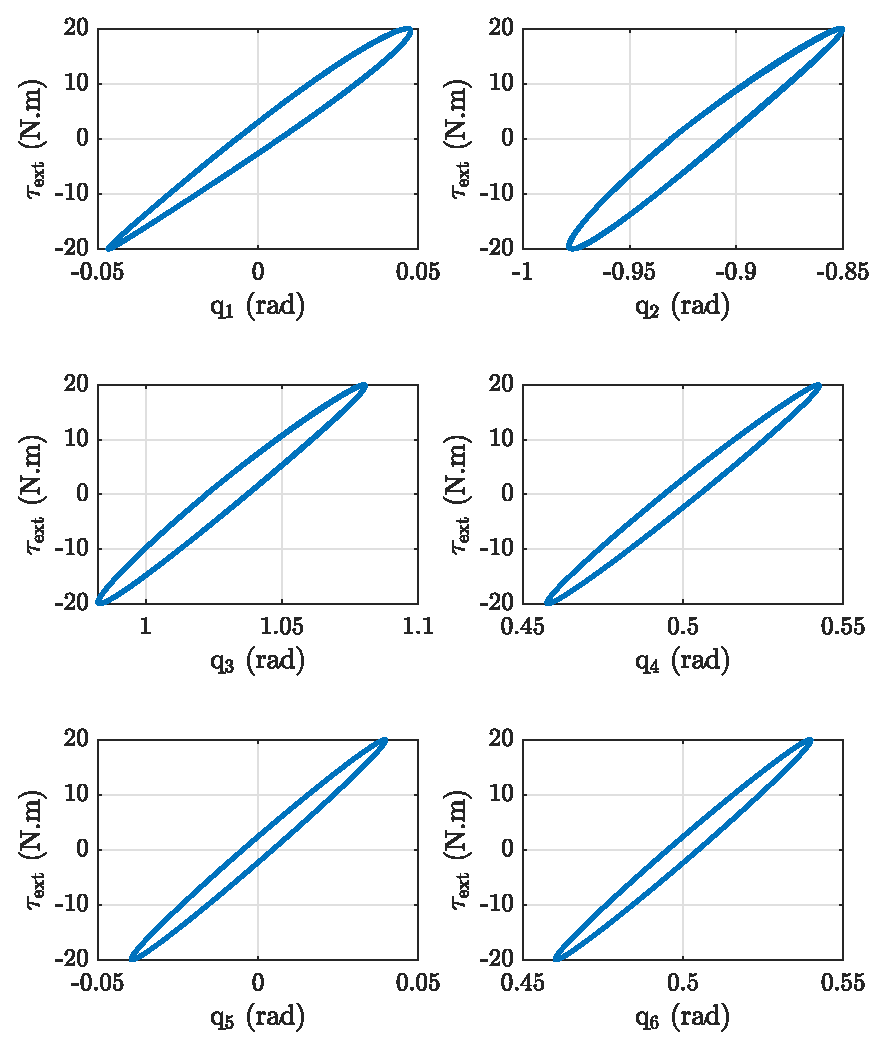
\includegraphics{external_torque_vs_joint_position.eps}
\caption{Dynamic relation between external torque ($\tauext$) and joint positions ($\mathbf{q}$) using proportional-derivative impedance control \eqref{eq:articular_PDi} with $\mathbf{K_{des}}=500\eye$ $\mathrm{\frac{N.m}{rad}}$ $\mathbf{D_{des}}=10\eye$ and $\mathrm{\frac{N.m.s}{rad}}$.}
\label{fig:act1.1.3_tau_vs_q}
\end{figure}

\begin{figure}
\centering
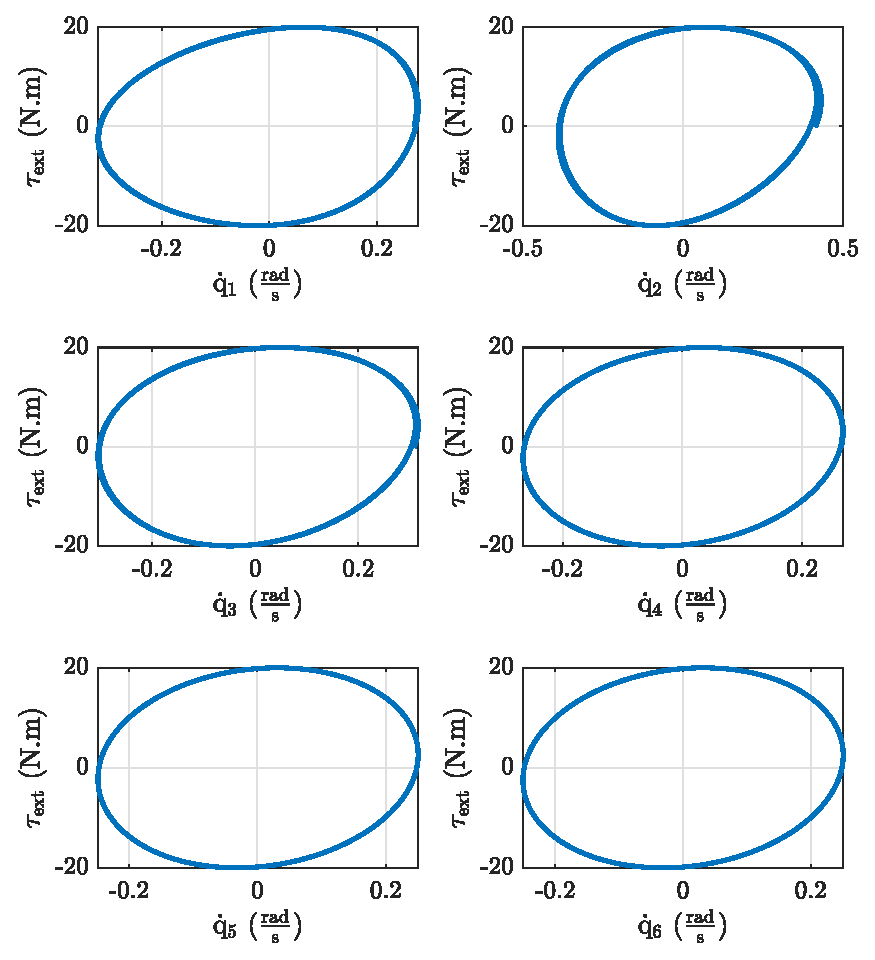
\includegraphics{external_torque_vs_joint_velocity.eps}
\caption{Dynamic relation between external torque ($\tauext$) and joint velocities ($\mathbf{\dot{q}}$) using proportional-derivative impedance control \eqref{eq:articular_PDi} with $\mathbf{K_{des}}=500\eye$ $\mathrm{\frac{N.m}{rad}}$ $\mathbf{D_{des}}=10\eye$ and $\mathrm{\frac{N.m.s}{rad}}$.}
\label{fig:act1.1.3_tau_vs_dq}
\end{figure}

\begin{figure}
\centering
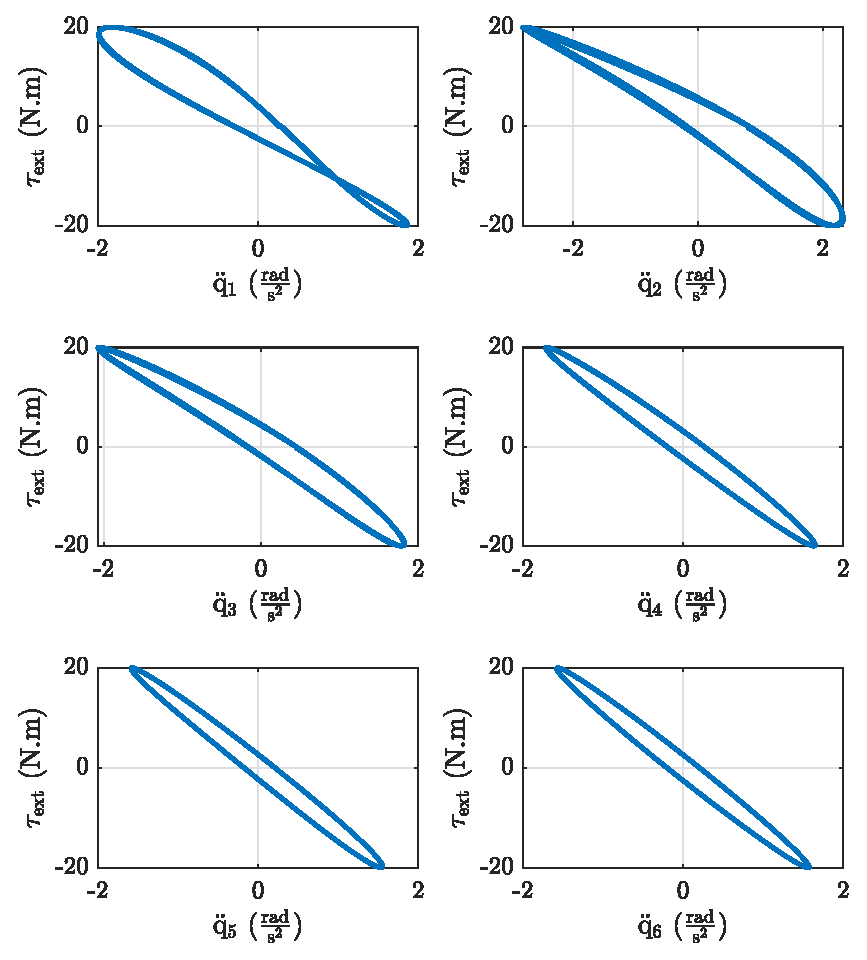
\includegraphics{external_torque_vs_joint_acceleration.eps}
\caption{Dynamic relation between external torque ($\tauext$) and joint accelerations ($\mathbf{\ddot{q}}$) using proportional-derivative impedance control \eqref{eq:articular_PDi} with $\mathbf{K_{des}}=500\eye$ $\mathrm{\frac{N.m}{rad}}$ $\mathbf{D_{des}}=10\eye$ and $\mathrm{\frac{N.m.s}{rad}}$.}
\label{fig:act1.1.3_tau_vs_ddq}
\end{figure}
